\section{Zofia Ficek}

\subsection{Carl Friedrich Gauss}

\hspace{\parindent} \textbf{Carl Friedrich Gauss} był niemieckim matematykiem, urodzonym w 1777 roku. Już w dzieciństwie wykazywał niezwykłe zdolności matematyczne, co zaowocowało jego późniejszymi osiągnięciami. Jego najważniejszym dziełem jest \textit{"Disquisitiones Arithmeticae"}, które zrewolucjonizowało teorię liczb. 
\par \textbf{Gauss} wprowadził pojęcie kongruencji oraz zajmował się badaniem liczb pierwszych. Jego prace w analizie matematycznej przyczyniły się do rozwoju teorii funkcji i równań różniczkowych. Znany jest również z analizy statystycznej, w tym z wprowadzenia rozkładu normalnego, zwanego krzywą Gaussa. Gauss zmarł w 1855 roku, pozostawiając po sobie niezatarte ślady w matematyce i nauce.
\par\noindent Poniżej (Rysunek \ref{fig:gauss}) portret uczonego
\begin{figure}[ht]
    \centering
    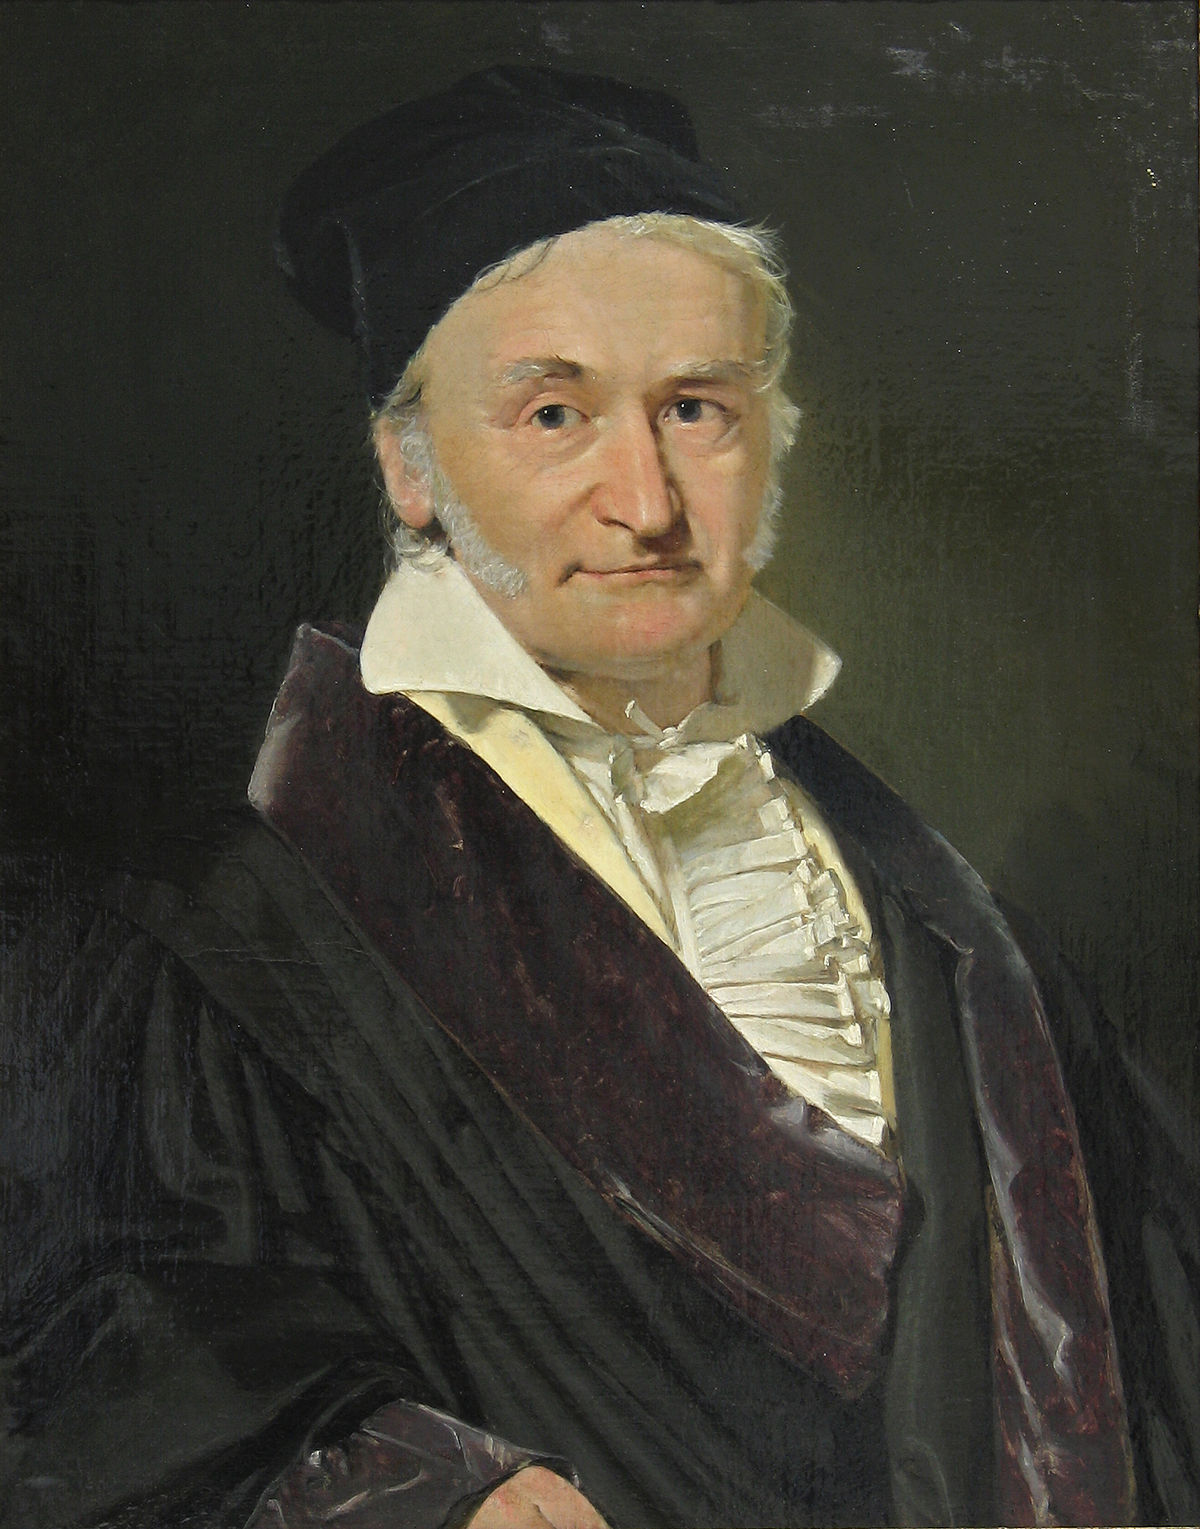
\includegraphics[width=0.5\textwidth]{pictures/gauss.jpg}
    \caption{Carl Friedrich Gauss}
    \label{fig:gauss}
\end{figure}

\subsection{Krzywa Gaussa}
\hspace{\parindent} \textbf{Krzywa Gaussa}, znana również jako krzywa normalna, to graficzne przedstawienie rozkładu normalnego. Jest to jeden z najważniejszych rozkładów w statystyce, charakteryzujący się symetrią i dzwonowatym kształtem
\par \textbf {Wzór krzywej Gaussa}, jest dany przez
\[f(x) = \frac{1}{\sigma \sqrt{2\pi}} e^{-\frac{(x - \mu)^2}{2\sigma^2}}\]
\begin{itemize}
    \renewcommand\labelitemi{--}
    \item $f(x)$ to wartość funkcji gęstości rozkładu dla punktu $x$
    \item \( \mu\) to średnia rozkładu
    \item \(\sigma\) to odchylenie standardowe
    \item $e$ to podstawa logarytmu naturalnego (około 2.71828)
    \item \(\pi\) to liczba Pi (około 3.14159)
\end{itemize}
\vspace{0,5cm} 
\par Kluczowe cechy \textbf{krzywej Gaussa}
\begin{enumerate}
    \item \textbf{Symetria}: Krzywa jest symetryczna względem swojej średniej, co oznacza, że wartości są równomiernie rozłożone po obu stronach.
    \item \textbf{Średnia, mediana, dominanta}: W rozkładzie normalnym te trzy miary centralne są sobie równe i znajdują się w punkcie szczytu krzywej.
    \item \textbf{Parametry}: Krzywa Gaussa jest określona przez dwa parametry: średnią \( \mu\) i odchylenie standardowe \(\sigma\). Średnia wskazuje, gdzie znajduje się środek rozkładu, a odchylenie standardowe określa, jak bardzo dane są rozproszone.
    \item \textbf{Zastosowania}: Powszechnie używana w statystyce, naukach przyrodniczych, ekonomii i wielu innych dziedzinach do modelowania danych i zjawisk losowych.
\end{enumerate}

\subsection{Nagroda Gaussa}
\par Nagroda Gaussa (Nagroda im. Carla Friedricha Gaussa) to prestiżowe wyróżnienie przyznawane przez Międzynarodową Unię Matematyczną (IMU) za wybitne osiągnięcia w dziedzinie matematyki. Nagroda jest często uważana za równoważną z innymi prestiżowymi wyróżnieniami w dziedzinie nauk, takimi jak Nagroda Nobla. Tabela \ref{tab:gauss} przedstawia daty i zdobywców Nagrody Gaussa:
\begin{table}[ht]
    \centering
    \begin{tabular}{|c|c|}
    \hline
    Rok & Zdobywca nagrody              \\
    \hline
    2006 & Jean-Pierre Serre            \\
    \hline
    2007 & S. R. Srinivasa Varadhan     \\
    \hline
    2008 & John G. Thompson             \\
    \hline
    2009 & Mikio Sato                   \\
    \hline
    2010 & John Nash                    \\
    \hline
    2011 & Goro Shimura                 \\
    \hline
    2012 & Alain Connes                 \\
    \hline
    2013 & Peter Scholze                \\
    \hline
    2014 & Andrew Wiles                 \\
    \hline
    2015 & Louis Nirenberg              \\
    \hline
    2016 & Jean Bourgain                \\
    \hline
    2017 & Robert Langlands             \\
    \hline
    2018 & Efim Zelmanov                \\
    \hline
    2019 & Michael Hopkins              \\
    \hline
    2020 & Hillel Furstenberg           \\
    \hline
    2021 & László Lovász                \\
    \hline
    2022 & June Huh                     \\
    \hline
    2023 & N/A                          \\
    \hline
    \end{tabular}
    \caption{Zadobywcy Nagrody Gaussa w latach 2006-2023}
    \label{tab:gauss}
\end{table}


